\documentclass[10pt]{article}
\usepackage{amsmath, amsthm, amsbsy, rotating,float}
\usepackage{graphicx,algorithm,algorithmic}
\usepackage{setspace,enumerate}
\usepackage[font=small,labelfont=bf]{caption}

\usepackage{graphicx,caption,subfig}

\floatstyle{ruled}
\newfloat{program}{thp}{lop}
\doublespacing


\def\dt{\delta t}
\def\dxs{{\delta x}^2}
\def\heq{\frac{\partial u}{\partial t} -a\frac{\partial^2 u}{\partial x^2}}

\def\up#1{ #1^{\prime}}


\def\intab#1{\int_{\alpha}^{\beta} #1 dx}
\def\evat{\bigg|_{\alpha}^{\beta}}

\author{Esteban D\'{i}az}
\title{Galerkin Finite Element Method for the 1D Poisson equation}{}

\begin{document}
\def\pcscwp{
Center for Wave Phenomena \\ 
Colorado School of Mines \\ 
psava@mines.edu
}

\def\pcscover{
\author[]{Paul Sava}
\institute{\pcscwp}
\date{}
\logo{WSI}
\large
}

\def\WSI{\textbf{WSI}~}

% ------------------------------------------------------------
% colors
\definecolor{darkgreen}{rgb}{0,0.4,0}
\definecolor{LightGray}{rgb}{0.90,0.90,0.90}
\definecolor{DarkGray}{rgb}{0.85,0.85,0.85}

\definecolor{LightGreen} {rgb}{0.792,1.000,0.439}
\definecolor{LightYellow}{rgb}{1.000,0.925,0.545}
\definecolor{LightBlue}  {rgb}{0.690,0.886,1.000}
\definecolor{LightRed}   {rgb}{1.000,0.752,0.796}
\definecolor{Blue} {rgb}{0,0.08,0.45}



\def\red#1{\textcolor{red}{#1}}
\def\blue#1{\textcolor{blue}{#1}}
\def\green#1{\textcolor{green}{#1}}
\def\darkgreen#1{\textcolor{darkgreen}{#1}}
\def\black#1{\textcolor{black}{#1}}
\def\white#1{\textcolor{white}{#1}}
\def\yellow#1{\textcolor{yellow}{#1}}
\def\gray#1{\textcolor{gray}{#1}}
\def\magenta#1{\textcolor{magenta}{#1}}

% ------------------------------------------------------------
% madagascar
\def\mg{\darkgreen{\sc madagascar~}}
\def\mex#1{ \red{ #1 } }
\def\mvbt#1{\small{\blue{\begin{semiverbatim}#1\end{semiverbatim}}}}

% ------------------------------------------------------------
% equations
\def\bea{\begin{eqnarray}}
\def\eea{  \end{eqnarray}}

\def\beq{\begin{equation}}
\def\eeq{  \end{equation}}

% Norm symbol
\newcommand{\norm}[1]{\left|\left|#1\right|\right|}


%\def\req#1{(\ref{#1})}

\def\lp{\left (}
\def\rp{\right)}

\def\lb{\left [}
\def\rb{\right]}

\def\pbox#1{ \fbox {$ \displaystyle #1 $}}

\def\non{\nonumber \\ \nonumber}
\def\lnorm#1{\lVert#1\rVert}
% ------------------------------------------------------------
% REFERENCE (equations and figures)
\def\rEq#1{Equation~\ref{eqn:#1}}
\def\req#1{equation~\ref{eqn:#1}}
\def\rEqs#1{Equations~\ref{eqn:#1}}
\def\reqs#1{equations~\ref{eqn:#1}}
\def\ren#1{\ref{eqn:#1}}

\def\rFg#1{Figure~\ref{fig:#1}}
\def\rfg#1{Figure~\ref{fig:#1}}
\def\rFgs#1{Figures~\ref{fig:#1}}
\def\rfgs#1{Figures~\ref{fig:#1}}
\def\rfn#1{\ref{fig:#1}}

% ------------------------------------------------------------
% field operators

% trace
\def\tr{\texttt{tr}\;}

% divergence
\def\DIV#1{\nabla \cdot {#1}}

% curl
\def\CURL#1{\nabla \times {#1}}

% gradient
\def\GRAD#1{\nabla {#1}}

% Laplacian
\def\LAPL#1{\nabla^2 {#1}}

\def\dellin{
\lb
\begin{matrix}
\done{}{x} \; \done{}{y} \; \done{}{z}
\end{matrix}
\rb
}

\def\delcol{
\lb
\begin{matrix}
\done{}{x} \non
\done{}{y} \non
\done{}{z}
\end{matrix}
\rb
}

\def\aveclin{
\lb
\begin{matrix}
a_x \; a_y \; a_z
\end{matrix}
\rb
}


% ------------------------------------------------------------

% elastic tensor
\def\CC{{\bf C}}

% identity tensor
\def\I{\;{\bf I}}

% particle displacement vector
\def\uu{{\bf u}}

% particle velocity vector
\def\vv{{\bf v}}

% particle acceleration vector
\def\aa{{\bf a}}

% force vector
\def\ff{{\bf f}}

% wavenumber vector
\def\kk{{\bf k}}

% ray parameter vector
\def\pp{{\bf p}}

% distance vector
\def\hh{ {\boldsymbol{\lambda}} }
\def\xx{{\bf x}}
\def\kkx{{\kk_\xx}}
\def\ppx{{\pp_\xx}}

\def\yy{{\bf y}}

% normal vector
\def\nn{{\bf n}}
\def\ns{\nn_s}
\def\nr{\nn_r}

% source vector
\def\ss{{\bf s}}
\def\kks{{\kk_\ss}}
\def\pps{{\pp_\ss}}

% receiver vector
\def\rr{{\bf r}}
\def\kkr{{\kk_\rr}}
\def\ppr{{\pp_\rr}}

% midpoint vector
\def\mm{{\bf m}}
\def\kkm{{\kk_\mm}}
\def\ppm{{\pp_\mm}}

% offset vector
\def\ho{{\bf h}}
\def\kkh{{\kk_\ho}}
\def\pph{{\pp_\ho}}

% space-lag vector

\def\kkl{{\kk_\hh}}
\def\ppl{{\pp_\hh}}

% CIP vector
\def\cc{ {\bf c}}

% time-lag scalar
\def\tt{\tau}
\def\tts{\tt_s}
\def\ttr{\tt_r}

% frequency
\def\ww{\omega}

%
\def\dd{{\bf d}}

\def\bb{{\bf b}}
\def\qq{{\bf q}}

\def\ii{{\bf i}} % unit vector
\def\jj{{\bf j}} % unit vector

\def\lo{{\bf l}}

% ------------------------------------------------------------

\def\Fop#1{\mathcal{F}     \lb #1 \rb}
\def\Fin#1{\mathcal{F}^{-1}\lb #1 \rb}


% ------------------------------------------------------------
% wave equation operators:

\def\swe#1{ \frac{1}{v^2(\xx)}\dtwo{#1}{t}- \LAPL{#1}}
\def\awe#1{ \frac{1}{v_p^2(\xx) \rho(\xx)}\dtwo{#1}{t}- \DIV{\frac{1}{\rho(\xx)}\GRAD{#1}} }
\def\ewe#1{ \rho(\xx) \dtwo{#1}{t} -v_p(\xx)^2\LAPL{#1}+v_s(\xx)^2\CURL{\CURL{#1}}}

% ------------------------------------------------------------
% partial derivatives

\def\dtwo#1#2{\frac{\partial^2 #1}{\partial #2^2}}
\def\done#1#2{\frac{\partial   #1}{\partial #2  }}
\def\dthr#1#2{\frac{\partial^3 #1}{\partial #2^3}}
\def\mtwo#1#2#3{ \frac{\partial^2#1}{\partial #2 \partial#3} }

\def\larrow#1{\stackrel{#1}{\longleftarrow}}
\def\rarrow#1{\stackrel{#1}{\longrightarrow}}

% ------------------------------------------------------------
% elasticity 

\def\stress{\underline{\textbf{t}}}
\def\strain{\underline{\textbf{e}}}
\def\stiffness{\underline{\underline{\textbf{c}}}}
\def\compliance{\underline{\underline{\textbf{s}}}}

\def\GEOMlaw{
\strain = \frac{1}{2} 
\lb \GRAD{\uu} + \lp \GRAD{\uu} \rp^T \rb
}

\def\HOOKElaw{
\stress = \lambda \; tr \lp \strain \rp {\bf I} + 2 \mu \strain 
}

\def\CONSTITUTIVElaw{
\stress = \stiffness \;\strain 
}


\def\NEWTONlaw{
\rho \ddot{\uu} = \DIV{\stress}
}

\def\NAVIEReq{
\rho \ddot\uu =
\lp \lambda + 2\mu \rp \GRAD{\lp \DIV{\uu} \rp}
             - \mu     \CURL{   \CURL{\uu}}
}

% ------------------------------------------------------------

% potentials
\def\VP{\boldsymbol{\psi}}
\def\SP{\theta}

% stress tensor
\def\ssten{{\bf \sigma}}

\def\ssmat{
\lp \matrix {
 \sigma_{11} &  \sigma_{12}   &  \sigma_{13} \cr
 \sigma_{12} &  \sigma_{22}   &  \sigma_{23} \cr
 \sigma_{13} &  \sigma_{23}   &  \sigma_{33} \cr
} \rp
}

% strain tensor
\def\eeten{{\bf \epsilon}}

\def\eemat{
\lp \matrix {
 \epsilon_{11} &  \epsilon_{12}   &  \epsilon_{13} \cr
 \epsilon_{12} &  \epsilon_{22}   &  \epsilon_{23} \cr
 \epsilon_{13} &  \epsilon_{23}   &  \epsilon_{33} \cr
} \rp
}


% plane wave kernel
\def\pwker{A e^{i k \lp \nn \cdot \xx - v t \rp}}


% ------------------------------------------------------------
% details for expert audience (math, cartoons)
\def\expert{
\colorbox{red}{\textbf{\LARGE \white{!}}}
}

% ------------------------------------------------------------
% image, data, wavefields

\def\RR{R}

\def\R{R(\xx)}
\def\Re{R(\xx,\hh,\tau)}
\def\Rc#1{R^{#1}(\xx)}
\def\Rce#1{R^{#1}(\xx,\hh,\tau)}
\def\Rct#1{R^{#1}(z,\tau)}
\def\Rcl#1{R^{#1}(z,\lambda_x)}

\def\UU{u}
\def\US{{\UU_s}}
\def\USt{{\UU_s^f}}
\def\USr{{\UU_s^b}}
\def\UR{{\UU_r}}
\def\URt{{\UU_r^f}}
\def\URr{{\UU_r^b}}

\def\DD{D}
\def\DS{{\DD_s}}
\def\DR{{\DD_r}}

\def\UUw{\UU}
\def\USw{{\UU_s}}
\def\URw{{\UU_r}}

\def\DDw{\DD}
\def\DSw{{\DD_s}}
\def\DRw{{\DD_r}}

% perturbations

\def\ds{\Delta s}
\def\di{\Delta \RR}
\def\du{\Delta \UU}

\def\dRR{\Delta \RR}
\def\dUU{\Delta \UU}
\def\dUS{\Delta \US}
\def\dUR{\Delta \UR}

\def\dtt{\Delta \tt}
\def\dhh{\Delta \hh}

% ------------------------------------------------------------
% Green's functions

\def\GG{G}

\def\GS{{\GG_s}}
\def\GR{{\GG_r}}

% ------------------------------------------------------------
% elastic data, wavefields

\def\eRR{\textbf{\RR}}

\def\eDS{{\textbf{\DD}_s}}
\def\eDR{{\textbf{\DD}_r}}
\def\eDD{{\textbf{\DD}}}

\def\eUS{{\textbf{\UU}_s}}
\def\eUR{{\textbf{\UU}_r}}
\def\eUU{{\textbf{\UU}}}

% ------------------------------------------------------------
% sliding bar
\def\tline#1{
\put(95,-3){\small \blue{time}}
\put(-4,-1){\small \blue{0}}
\thicklines
\put( 0,0){\color{blue} \vector(1,0){100}}
\put(#1,0){\color{red}  \circle*{2}}
}

% ------------------------------------------------------------
% arrow on figure
\def\myarrow#1#2#3{
\thicklines
\put(#1,#2){\color{green} \vector(-1,-1){5}}
\put(#1,#2){\color{green} \textbf{#3}}
}

\def\bkarrow#1#2#3{
\thicklines
\put(#1,#2){\color{black} \vector(-1,-1){5}}
\put(#1,#2){\color{black} \textbf{#3}}
}


\def\anarrow#1#2#3#4{
\thicklines
\put(#1,#2){\color{#4} \vector(-1,-1){5}}
\put(#1,#2){\color{#4} \textbf{#3}}
}

% ------------------------------------------------------------
% circle on figure
\def\mycircle#1#2#3{
\thicklines
\put(#1,#2){\color{green} \circle{#3}}
}

% ------------------------------------------------------------
% note on figure
\def\mynote#1#2#3{
\put(#1,#2){\color{green} \textbf{#3}}
}

\def\biglabel#1#2#3{
\put(#1,#2){\Huge \textbf{#3}}
}

\def \largelabel#1#2#3{
\put(#1,#2){\Large \textbf{#3}}
}


\def \normallabel#1#2#3{
\put(#1,#2){\normalsize \textbf{#3}}
}




\def\waxes{\put(-0,0){\color{white}\vector(1,0){10}}
\color{white} \klabellarge{10.5}{-1}{\color{white} {x}}
\put(-0,0){\color{white} \vector(0,-1){10}}
\color{white} \klabellarge{-1.2}{-14.5}{\color{white} {z}}}


\def\axes{\put(-0,0){\vector(1,0){10}}
\klabellarge{10.5}{-1}{\bf{x}}
\put(-0,0){\vector(0,-1){10}}
\klabellarge{-1.2}{-14.5}{\bf{z}}}



\def\putaxes#1#2{\put(#1,#2){\axes}}
\def\putwaxes#1#2{\put(#1,#2){\waxes}}

% huge labels
\def\wlabel#1#2#3{ \white{ \biglabel{#1}{#2}{#3} }}
\def\klabel#1#2#3{ \black{ \biglabel{#1}{#2}{#3} }}
\def\rlabel#1#2#3{ \red{   \biglabel{#1}{#2}{#3} }}
\def\glabel#1#2#3{ \green{ \biglabel{#1}{#2}{#3} }}
\def\blabel#1#2#3{ \blue { \biglabel{#1}{#2}{#3} }}
\def\ylabel#1#2#3{ \yellow{\biglabel{#1}{#2}{#3} }}


% large labels
\def\klabellarge#1#2#3{ \black{ \largelabel{#1}{#2}{#3} }}
\def\wlabellarge#1#2#3{ \white{ \largelabel{#1}{#2}{#3} }}

% normal labels
\def\klabelnormal#1#2#3{ \black{ \normallabel{#1}{#2}{#3} }}
\def\wlabelnormal#1#2#3{ \white{ \normallabel{#1}{#2}{#3} }}

% ------------------------------------------------------------
% centering
\def\cen#1{ \begin{center} \textbf{#1} \end{center}}
\def\cit#1{ \begin{center} \textit{#1} \end{center}}

% emphasis (bold+alert)
\def\bld#1{ \textbf{\alert{#1}}}

% huge fonts
\def\big#1{\begin{center} {\LARGE \textbf{#1}} \end{center}}
\def\hug#1{\begin{center} {\Huge  \textbf{#1}} \end{center}}

% ------------------------------------------------------------
% separator
\def\sep{ \vfill \hrule \vfill}
\def\itab{ \hspace{0.5in}}
\def\nsp{\\ \vspace{0.1in}}

% ------------------------------------------------------------
% integrals

\def\tint#1{\!\!\!\int\!\! #1 dt}
\def\xint#1{\!\!\!\int\!\! #1 d\xx}
\def\wint#1{\!\!\!\int\!\! #1 d\ww}
\def\aint#1{\!\!\!\alert{\int}\!\! #1 d\alert{\xx}}

\def\esum#1{\sum\limits_{#1}}
\def\eint#1{\int\limits_{#1}}

% ------------------------------------------------------------
\def\CONJ#1{\overline{#1}}
\def\MOD#1{\left| {#1} \right|}

% ------------------------------------------------------------
% imaging components

\def\IC{\colorbox{yellow}{\textbf{I.C.}}\;}
\def\WR{\colorbox{yellow}{\textbf{W.R.}}\;}
\def\WE{\colorbox{yellow}{\textbf{W.E.}}\;}
\def\SO{\colorbox{yellow}{\textbf{SOURCE}}\;}
\def\WS{\colorbox{yellow}{\textbf{W.S.}}\;}

% ------------------------------------------------------------
% summary/take home message
\def\thm{take home message}

% ------------------------------------------------------------
\def\dx{\Delta x}
\def\dy{\Delta y}
\def\dz{\Delta z}
\def\dt{\Delta t}

\def\dhx{\Delta h_x}
\def\dhy{\Delta h_y}

\def\kz{{k_z}}
\def\kx{{k_x}}
\def\ky{{k_y}}

\def\kmx{k_{m_x}}
\def\kmy{k_{m_y}}
\def\khx{k_{h_x}}
\def\khy{k_{h_y}}

\def\why{ \alert{\widehat{{\khy}}}}
\def\whx{ \alert{\widehat{{\khx}}}}

\def\lx{{\lambda_x}}
\def\ly{{\lambda_y}}
\def\lz{{\lambda_z}}

\def\klx{k_{\lambda_x}}
\def\kly{k_{\lambda_y}}
\def\klz{k_{\lambda_z}}

\def\mx{{m_x}}
\def\my{{m_y}}
\def\mz{{m_z}}
\def\hx{{h_x}}
\def\hy{{h_y}}
\def\hz{{h_z}}

\def\sx{{s_x}}
\def\sy{{s_y}}
\def\rx{{r_x}}
\def\ry{{r_y}}

% ray parameter (absolute value)
\def\modp#1{\left| \pp_{#1} \right|}

% wavenumber
\def\modk#1{\left| \kk_{#1} \right|}

% ------------------------------------------------------------
\def\kzwk{ {\kz^{\kk}}}
\def\kzwx{ {\kz^{\xx}}}
 
\def\PSk#1{e^{\red{#1 i \kzwk \dz}}}
\def\PSx#1{e^{\red{#1 i \kzwx \dz}}}
\def\PS#1{ e^{\red{#1 i k_z   \dz}}}

\def\TT{t}
\def\TS{t_s}
\def\TR{t_r}

\def\oft{\lp t \rp}
\def\ofw{\lp \ww \rp}

\def\ofx{\lp \xx \rp}
\def\ofk{\lp \kk \rp}
\def\ofs{\lp \ss \rp}
\def\ofr{\lp \rr \rp}
\def\ofz{\lp   z \rp}

\def\ofxt{\lp \xx, t  \rp}
\def\ofst{\lp \ss, t  \rp}
\def\ofrt{\lp \rr, t  \rp}

\def\ofxw{\lp \xx, \ww  \rp}
\def\ofsw{\lp \ss, \ww  \rp}
\def\ofrw{\lp \rr, \ww  \rp}

\def\ofxm{\lp \xx,\hh \rp}

\def\ofxmp{\lp \xx+\hh \rp}
\def\ofxmm{\lp \xx-\hh \rp}

\def\ofmm{\lp \mm      \rp}
\def\ofmz{\lp \mm, z   \rp}
\def\ofmw{\lp \mm, \ww \rp}
\def\ofkm{\lp \kkm     \rp}

% ------------------------------------------------------------
% source/receiver data and wavefields

\def\dst{$\DS\ofst$}
\def\drt{$\DR\ofrt$}
\def\ust{$\US\ofxt$}
\def\urt{$\UR\ofxt$}

\def\dsw{$\DS\ofsw$}
\def\drw{$\DR\ofrw$}
\def\usw{$\US\ofxw$}
\def\urw{$\UR\ofxw$}

% ------------------------------------------------------------
\def\Nx{N_x}
\def\Ny{N_y}
\def\Nz{N_z}
\def\Nt{N_t}
\def\Nw{N_{\ww}}
\def\Nm{N_{\mm}}

\def\Nlx{N_{\lambda_x}}
\def\Nly{N_{\lambda_y}}
\def\Nlz{N_{\lambda_z}}
\def\Nlt{N_{\tau}}

\def\wmin{\ww_{min}}
\def\wmax{\ww_{max}}
\def\zmin{z_{min}}
\def\zmax{z_{max}}
\def\tmin{t_{min}}
\def\tmax{t_{max}}
\def\lmin{\hh_{min}}
\def\lmax{\hh_{max}}
\def\xmin{\xx_{min}}
\def\xmax{\xx_{max}}

% ------------------------------------------------------------
% course qualifiers

\def\fun{\hfill \alert{concepts}}
\def\pra{\hfill \alert{applications}}
\def\fro{\hfill \alert{frontiers}}


% ------------------------------------------------------------
% wavefield extrapolation
\def\ws{ {\ww s} }

\def\kows{\lp \frac{\kx}{\ws} \rp}

\def\kmws{\lp \frac{\modk{\mm}}{\ws} \rp}
\def\kzws{\lp \frac{\kz}       {\ws} \rp}

\def\S{\lb\frac{\modk{\mm}}{\ws  }\rb}
\def\C{\lb\frac{\modk{\mm}}{\ws_0}\rb}
\def\K{\lb\frac{\modk{\mm}}{\ww  }\rb}

\def\Cs{\lb\frac{\modk{\mm}^2}{\lp \ws_0 \rp^2}\rb}

\def\SSR#1{  \sqrt{ \lp \ww {#1} \rp^2 - \modk{\mm}^2} }

\def\SQRsum#1{\sum\limits_{n=1}^{\infty} \lp -1 \rp^n
		\displaystyle{\frac{1}{2} \choose n} #1}

\def\TSE#1#2#3#4{\sum\limits_{#4=#3}^{\infty} \lp -1 \rp^#4
		\displaystyle{#2 \choose #4} {#1}^#4}

\def\onefrac#1#2{\frac{#2^2}{a_#1+b_#1 #2^2}}
\def\SQRfrac#1{
	\sum\limits_{n=1}^{\infty}
	\onefrac{n}{#1} }

\def\dkzds { \left. \frac{d {\kz}}  {d s} \right|_{s_b} }
\def\SSX#1#2{\sqrt{ 1 - \lb \frac{\MOD{#2}}{#1} \rb^2} }
\def\SST#1#2{1 + \sum_{j=1}^N c_j \lb \frac{\MOD{#2}}{#1} \rb^{2j} }

% ------------------------------------------------------------
% acknowledgment
\def\ackcwp{\cen{the sponsors of the\\Center for Wave Phenomena\\at\\Colorado School of Mines}}

% ------------------------------------------------------------
% citation in slides
\def\talkcite#1{{\small \sc #1}}

% ------------------------------------------------------------
\def\ise{GPGN302: Introduction to Electromagnetic and Seismic Exploration}
\def\inv{GPGN409: Inversion}

% ------------------------------------------------------------
\def\model{m}
\def\data {d}

\def\Lop{ {\mathbf{L}}}
\def\Sop{ {\mathbf{S}}}
\def\Eop{ {\mathbf{E}}}
\def\Iop{ {\mathbf{I}}}
\def\Aop{ {\mathbf{A}}}
\def\Pop{ {\mathbf{P}}}
\def\Fop{ {\mathbf{F}}}


% ------------------------------------------------------------
\def\mybox#1{
  \begin{center}
    \fcolorbox{black}{yellow}
    {\begin{minipage}{0.8\columnwidth} {#1} \end{minipage}}
  \end{center}
}

\def\hibox#1{
  \begin{center}
    \fcolorbox{black}{LightGreen}
    {\begin{minipage}{0.8\columnwidth} {#1} \end{minipage}}
  \end{center}
}

% ------------------------------------------------------------
% Nota Bene
\def\nbnote#1{
  \vfill
  \begin{center}
    \colorbox{LightGray}
    {\begin{minipage}{\columnwidth} {\textbf{\black{\large N.B.}} #1} \end{minipage}}
  \end{center}
}

\def\highlight#1{
  \begin{center}
    \colorbox{cyan}
    {\begin{minipage}{\columnwidth} {#1} \end{minipage}}
  \end{center}
}

% ------------------------------------------------------------
\def\pcsshaded#1{
  \definecolor{shadecolor}{rgb}{0.8,0.8,0.8}
  \begin{shaded} {#1} \end{shaded}
  \definecolor{shadecolor}{rgb}{1.0,1.0,1.0}
}

% ------------------------------------------------------------
\def\postit#1{
  \begin{center}
    \colorbox{yellow}
    {\begin{minipage}{0.66\columnwidth} {#1} \end{minipage}} 
  \end{center}
}

% ------------------------------------------------------------
\def\graybox#1{
  \begin{center}
    \colorbox{LightGray}
    {\begin{minipage}{1.00\columnwidth} {#1} \end{minipage}}
  \end{center}
}

\def\whitebox#1{
  \begin{center}
    \colorbox{white}
    {\begin{minipage}{1.00\columnwidth} {#1} \end{minipage}}
  \end{center}
}

\def\yellowbox#1{
  \begin{center}
    \colorbox{LightYellow}
    {\begin{minipage}{1.00\columnwidth} {#1} \end{minipage}}
  \end{center}
}

\def\greenbox#1{
  \begin{center}
    \colorbox{LightGreen}
    {\begin{minipage}{1.00\columnwidth} {#1} \end{minipage}}
  \end{center}
}

\def\bluebox#1{
  \begin{center}
    \colorbox{LightBlue}
    {\begin{minipage}{1.00\columnwidth} {#1} \end{minipage}}
  \end{center}
}

\def\redbox#1{
  \begin{center}
    \colorbox{LightRed}
    {\begin{minipage}{1.00\columnwidth} {#1} \end{minipage}}
  \end{center}
}

\def\hyellow#1{ \colorbox{yellow} #1 }
\def\hgreen #1{ \colorbox{green}  #1 }

% ------------------------------------------------------------
% boxes for vectors and matrices

\def\pcsbox#1#2#3#4{
  % #1 = width
  % #2 = height
  % %3 = hmax
  \begin{picture}(#3,#1)
    \linethickness{0.5mm}
    % 
    \multiput(0,#1)(#3, 0){2}{\line(0,-1){#2}}
    \multiput(0,#1)(0,-#2){2}{\line(+1,0){#3}}
    % 
    \put(1,3){#4}
  \end{picture}
}

\def\pcssym#1#2{
  \begin{picture}(1,#1)
    \put(0,3){#2}
  \end{picture}
}

\def\sidebyside#1#2{
  \begin{center}
    \colorbox{LightBlue}{
      \begin{minipage}{1.0\columnwidth} {#1} \end{minipage}
    }
    \colorbox{LightYellow}{
      \begin{minipage}{1.0\columnwidth} {#2} \end{minipage}
    }
  \end{center}
}

\def\sidebysidebyside#1#2#3{
  \begin{center}
    \colorbox{LightBlue}{
      \begin{minipage}{1.0\columnwidth} {#1} \end{minipage}
    }
    \colorbox{LightYellow}{
      \begin{minipage}{1.0\columnwidth} {#2} \end{minipage}
    }
    \colorbox{LightRed}{
      \begin{minipage}{1.0\columnwidth} {#3} \end{minipage}
    }
  \end{center}
}


\maketitle
In this report we concentrate in the solutions for the Poisson equation
\beq
-\nabla\cdot(\sigma\nabla u) = g,\text{    in  } \Omega,
\label{eq:poisson}
\eeq
where $\sigma$ satisfies $0<\sigma_{min} \leq\sigma(x) \leq \sigma_{max}$, $\forall x \in \Omega$.

In this report we consider the 1D version of equation~\ref{eq:poisson}. Instead of solving the Poisson equation
explicitly or implicitly as in FD methods, we solve an equivalent problem which in 1d has the following form:
\beq
-\intab{ \up{\left(\sigma\up{u}\right)}v} = \intab{gv},
\label{eq:peq}
\eeq
where $v$ is a test function which belongs to the same space as $u$. In 1D $\Omega =(\alpha,\beta)$

Integrating by parts the left hand side of equation~\ref{eq:peq} results in:
\beq
\intab{ \sigma\up{u} \up{v} } - \sigma\up{u}v\evat = \intab{gv}.
\label{eq:weakform}
\eeq

Note that solving equation~\ref{eq:weakform} does not require to differentiate $\sigma$ and neither differentiate twice $u$. 
Therefore, $u$ is required to be once differentiable and so does $v$. A suitable space for $u,v$ is $H^1$. However, depending 
on the boundary conditions (BC), we might need to restrict the solutions to $H^1_0$. Therefore, for either case
$u,v$ and $\up{u},\up{v}$ need to have compact support.

We can rewrite equation~\ref{eq:weakform} as:
\beq
a(u,v) -\sigma\up{u}{v}\evat = F(v).
\label{eq:weakform}
\eeq

Here, $a(u,v) = \intab{ \sigma\up{u} \up{v} }$ is the bilinear form.
The test function v is arbitrary chosen, it has to be such that $v \in V \subset H^1$ or $v \in V \subset H^1_0$ depending
on the BC of $u$. In our case we choose as basis the ``hat function''. Therefore,
\beq
V  = span\{\phi_j : i=1,2,...,N\}
\eeq

So, we can write equation~\ref{eq:weakform} as:
\beq
a(u,\phi_j) -\sigma\up{u}{\phi_j}\evat = F(\phi_j).
\label{eq:weakform2}
\eeq

Since $u \in V$, then we can write it as a linear combination of the functions in $V$, this is:
\beq
u_h(x) = \sum_{i=1}^{N} \alpha_i \phi_i(x),
\label{eq:lin}
\eeq
Where $\alpha_i$ are the weights.

Due to the bilinear form of $a(.,.)$ we can rewrite equation~\ref{eq:weakform2} as
\beq
\sum_{i=1}^{N} \alpha_i\left(a(\phi_i,\phi_j) -\sigma\up{\phi_i}{\phi_j}\evat\right) = F(\phi_j).
\label{eq:weakform3}
\eeq

So, given a discretization of $\Omega = (\alpha,\beta)$ we can have the system of linear equations, which
reads:

\beq
  \left( {\bf A} + {\bf B}_1 \right) \vec{\alpha} = \vec{{F}} + \vec{{B}_2},
\label{eq:general}
\eeq
where ${\bf B}_1$ and $\vec{B}_2$ are related to the boundary conditions. This
stiffness matrix (lhs) is sparse and SPD; therefore, it can be efficiently solved using a Cholesky
decomposition.


Given a discretization of $\Omega$ of the form:
\[
\alpha=x_0 < x_1 < x_2 < x_3 < ... < x_{n-1} < x_n = \beta.
\]
$\phi_i$ can defined as:

\beq
\phi_i(x) = \left\{
     \begin{array}{lr}
       0  &: \alpha \leq x < x_{i-1} \\
       \frac{x - x_{i-−1}}{h_i} & : x_{i-1} \leq x < x_{i} \\
       \frac{x_{i+1}-−x}{h_{i+1}} & : x_{i} \leq x < x_{i+1} \\
       0  &: x_{i+1}\leq x \leq \beta \\
     \end{array}
   \right.
\eeq
where $h_i = x_i - x_{i-1}$. Note that $\phi_i(x_i) = 1$.

\begin{figure}
\includegraphics[width=0.8\textwidth]{fig/basis.pdf}
\caption{Basis functions $\phi_{i-1}(x),\phi_{i}(x),\phi_{i+1}(x)$.}
\label{fig:basis}
\end{figure}


Figure~\ref{fig:basis} shows the basis function for 3 contiguous points. Note that 
for any given interval only two functions exists, and $\phi_{i-1}(x) + \phi_{i}(x) = 1.$.

Once we solve for the weights $\alpha_i$ and having the base $V$ defined,
\beq
u_h(x) = \sum_i \alpha_i \phi_i(x).
\label{eq:uh}
\eeq
 If we happen to know the function we want to solve, then we can define an error functional
based on the $L_2$ norm which reads
\beq
\norm{u(x) - u_h(x)} = \sqrt{\intab{(u(x) - u_h(x))^2}}
\eeq



\section{Problem 1: Dirichlet BVP}

Here we want to solve:
\beq
-\nabla\cdot(\sigma\nabla u) = g,\text{    in  } \Omega=(\alpha,\beta), u=0\text{ on } \delta\Omega 
\label{eq:Dirichlet}
\eeq
where $\sigma$ satisfies the same conditions as in equation~\ref{eq:poisson}.

Since $u(\alpha)=u(\beta)=0$, then we choose a suitable base accordantly. Therefore, in this
problem $u,v \in V \subset H^1_0$ which means that both $u,v$ vanish at the bounds of the domain.

Considering that we know the endpoints of the discretized domain, we have to solve for 
$i=1,n$. The system of equations resulting from this BC is:
\beq
 {\bf A} \vec{\alpha} = \vec{{F}},
\label{eq:sdir}
\eeq
where ${\bf A}_{ij} = a(\phi_i,\phi_j), i=1,N$.

To further test the method implementation, I do numerical tests. The parameters for the tests are chosen
such that $u(x) = \sin(x)$:
\[
\sigma(x) = x+1,
\]
\[
g(x) = (1+x)\sin(x) -\cos(x)
\]
\[
u(0) = u(\pi) = 0
\]
To test the code, I use a regular grid with $n=100$, so $h = \phi/100$. I then evaluate the FEM solution
following equation~\ref{eq:uh}. Note that evaluating the FEM solution is equivalent to perform a linear
interpolation between two known points $u_i,u_{i+1}$, so our choice for $V$ acts as a linear interpolant on $\Omega$.

Figure~\ref{fig:fig1} shows the retrieved solution overlay with the true function (top) and the associated error.
Note that the error is oscillatory, this is due to our choice for the basis function. Basically what we see 
here is an interpolation error, where the error increases between the inverted control points $x_i$.

I then numerically explore the convergence properties of the method by changing the number of points in the grid:
$N = 2^k 100, k=0,1,2,3,4$. The results are shown in table~\ref{tab:table1}. The rate was calculated for 
each k as $r_k = \log(L2_{k-1}/L2_k)/\log(2)$. The rate is close to $r=2$ which is the expected rate given
the linear interpolant error. 


\begin{figure}
\centering
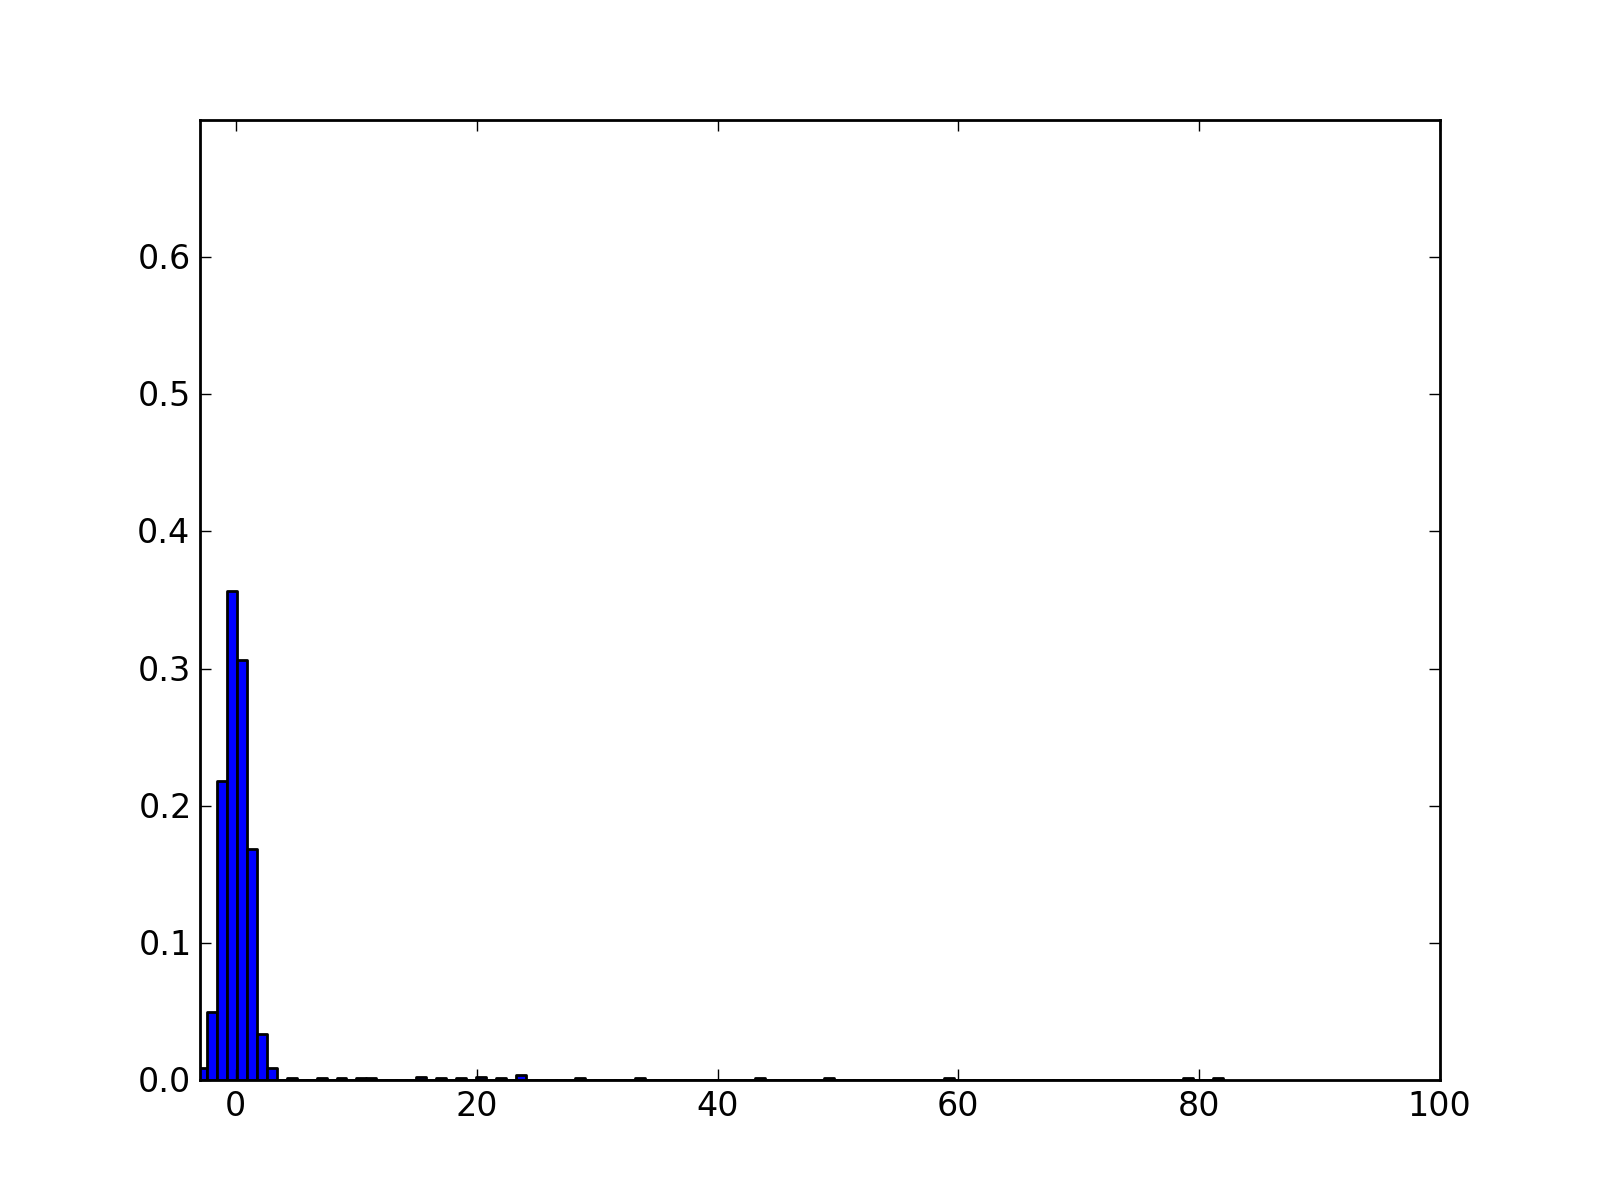
\includegraphics[width=0.6\textwidth]{fig/fig1.png}
\caption{Overlay of the FEM solution and $u(x)= \sin(x)$ (top), and error $e(x) = u(x)-u_h(x)$ (bottom).}
\label{fig:fig1}
\end{figure}

\begin{table}
\centering
  \begin{tabular}{c | c | c | c | c}
k&   N &      h    &     L2    &     rate       \\ \hline
0&  101& 0.03141593& 0.0001080497&     ---      \\
1&  201& 0.01570796& 2.703994e-05&  1.9985312   \\
2&  401& 0.00785398& 6.7599883e-06&  1.9999993  \\
3&  801& 0.00392699& 1.6899967e-06&  2.0000003  \\
4& 1601& 0.00196350& 4.2249092e-07&  2.0000282
  \end{tabular}
\caption{Convergence analysis for FEM method, problem 1.}
\label{tab:table1}
\end{table}



\section{Problem 2: Dirichlet-Neumman BVP}
Here we want to solve the problem:
\beq
-\nabla\cdot(\sigma\nabla u) = g,\text{    in  } \Omega=(\alpha,\beta), u(\alpha)=0, \up{u}(\beta) =\gamma
\label{eq:D-N}
\eeq

Here, $V$ is in $H^1$. The discretization of this problem is the same as the previous one. 
Here we have $N+1$ unknowns (we only know $u(0)=0$). Therefore, the weak form for this problem is that
of equation~\ref{eq:weakform3}.

Inserting the boundary condition data results in the following linear system:
\beq
 \left({\bf A} + {\bf B1}\right)\vec{\alpha} = \vec{{F}},
\label{eq:sdn}
\eeq

Where ${\bf B1}_{ij} = -\sigma\up{\phi}_i\phi_j (\beta)$. Note that 
the BC matrix only has one entry at ${\bf B1}_{N+1,N+1} = -\sigma(\beta)\up{u}(\beta)$. 

To test this BC we solve the problem such that $u(x) = \sin(2x) \in \Omega(0,\pi/4)$ with $\sigma(x) =1$. This results in:
$g(x) = 4\sin(2x)$, $\gamma = 0$.

In order to test the code, I create an uniform partition of $\Omega$, with $h = \pi/400$.
Figure~\ref{fig:fig2} shows the FEM solution for this problem with an overlay of the true answer (top), and the
associated error. One can see that the error is oscillatory, again this is related with the linear interpolant error
asscociated with our choice for the space. Here $u(x) > u_h(x)$.

Table~\ref{tab:table2} shows the convergence for this problem. To test the decay in the error, I 
change $N = 2^k100, k=0,1,2,3,4$. The rate is calculated in the same way as in previous problem. The 
estimated rate is $r=2$ which is consistent with the linear interpolant error.

\begin{figure}
\centering

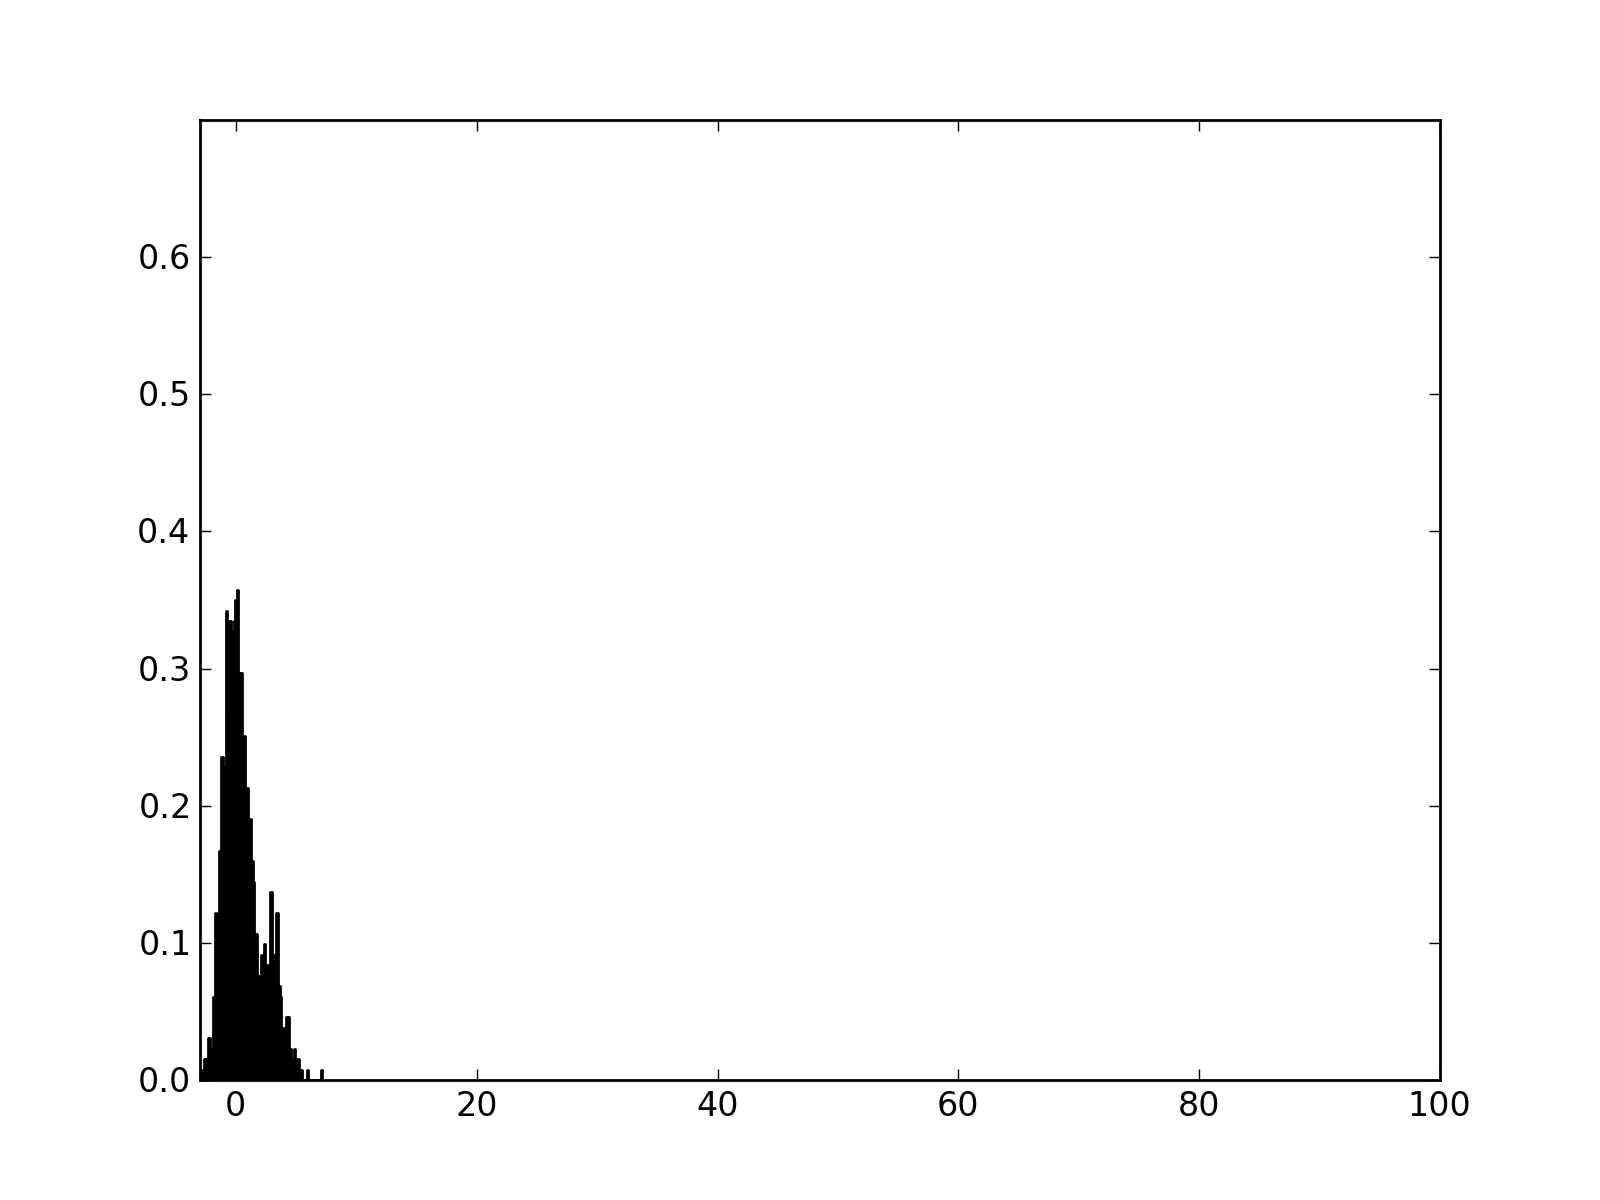
\includegraphics[width=0.6\textwidth]{fig/fig2.png}
\caption{Overlay of the FEM solution and $u(x)= 4\sin(2x)$ (top), and error $e(x) = u(x)-u_h(x)$ (bottom).}
\label{fig:fig2}
\end{figure}

\begin{table}
\centering
  \begin{tabular}{c | c | c | c | c}
k&   N &      h    &     L2    &     rate      \\ \hline
0&  101& 0.00785398& 1.4353305e-05&  --        \\
1&  201& 0.00392699& 3.5541949e-06&  2.0137882 \\
2&  401& 0.00196350& 8.850103e-07&  2.0057567  \\
3&  801& 0.00098175& 2.2079196e-07&  2.0030066 \\ 
4& 1601& 0.00049087& 5.5129197e-08&  2.0017991
  \end{tabular}
\caption{Convergence analysis for FEM method with D-N BC.}
\label{tab:table2}
\end{table}


\section{Problem 3: mixed BVP}
We now solve the following problem:
\beq
-\nabla\cdot(\sigma\nabla u) = g,\text{    in  } \Omega=(\alpha,\beta), \up{u}(\alpha)=3, \sigma(\beta)\up{u}(\beta) =\gamma -u(\beta).
\label{eq:Robin}
\eeq
Here, we know the flux in one side of the domain, and we know $\sigma(\beta)\up{u}(\beta)$ on the other side of the domain. 
We now have $N+2$ unknowns on the domain (we have to find the solution for $x_0$ and $x_{N+1}$). A suitable space
for this problem is $H^1$.

Here, the system of equations has the general form of equation~\ref{eq:general}, with 
${\bf B}_{ij},\text{  }i,j=0,...,N+1$ being a sparse matrix with one entry: ${\bf B}_{N+1,N+1} = 1$ 
and the vector $\vec{B2}$ has two entries:
\[
B2_{0,0} = -\sigma(\alpha)\up{u}(\alpha)
\]
and
\[
B2_{N+1,N+1} = \sigma(\beta)\gamma
\]


To test the implementation, I set up a problem with parameters chosen such that $\sigma(x)=1$ and $u(x) =\exp(3x)$. This
results in $g(x) = -9\exp(3x)$ and $\gamma=4\exp(3)$.

Similar to previous exercises, I test the implementation with $N=100$, and the interpolated solution $u_h$ evaluated
at 1000 points. Figure~\ref{fig:fig3} shows the retrieved solution, note that in this case $u(x) < u_h(x)$. 


To test the convergence, I change the number of points on the interval. Table~\ref{tab:table3} shows the results,
similar to Problems 1 and 2, the convergence rate is $r=2$ which is consistent with the linear interpolant
associated with our choice of $V$. 

\begin{figure}
\centering
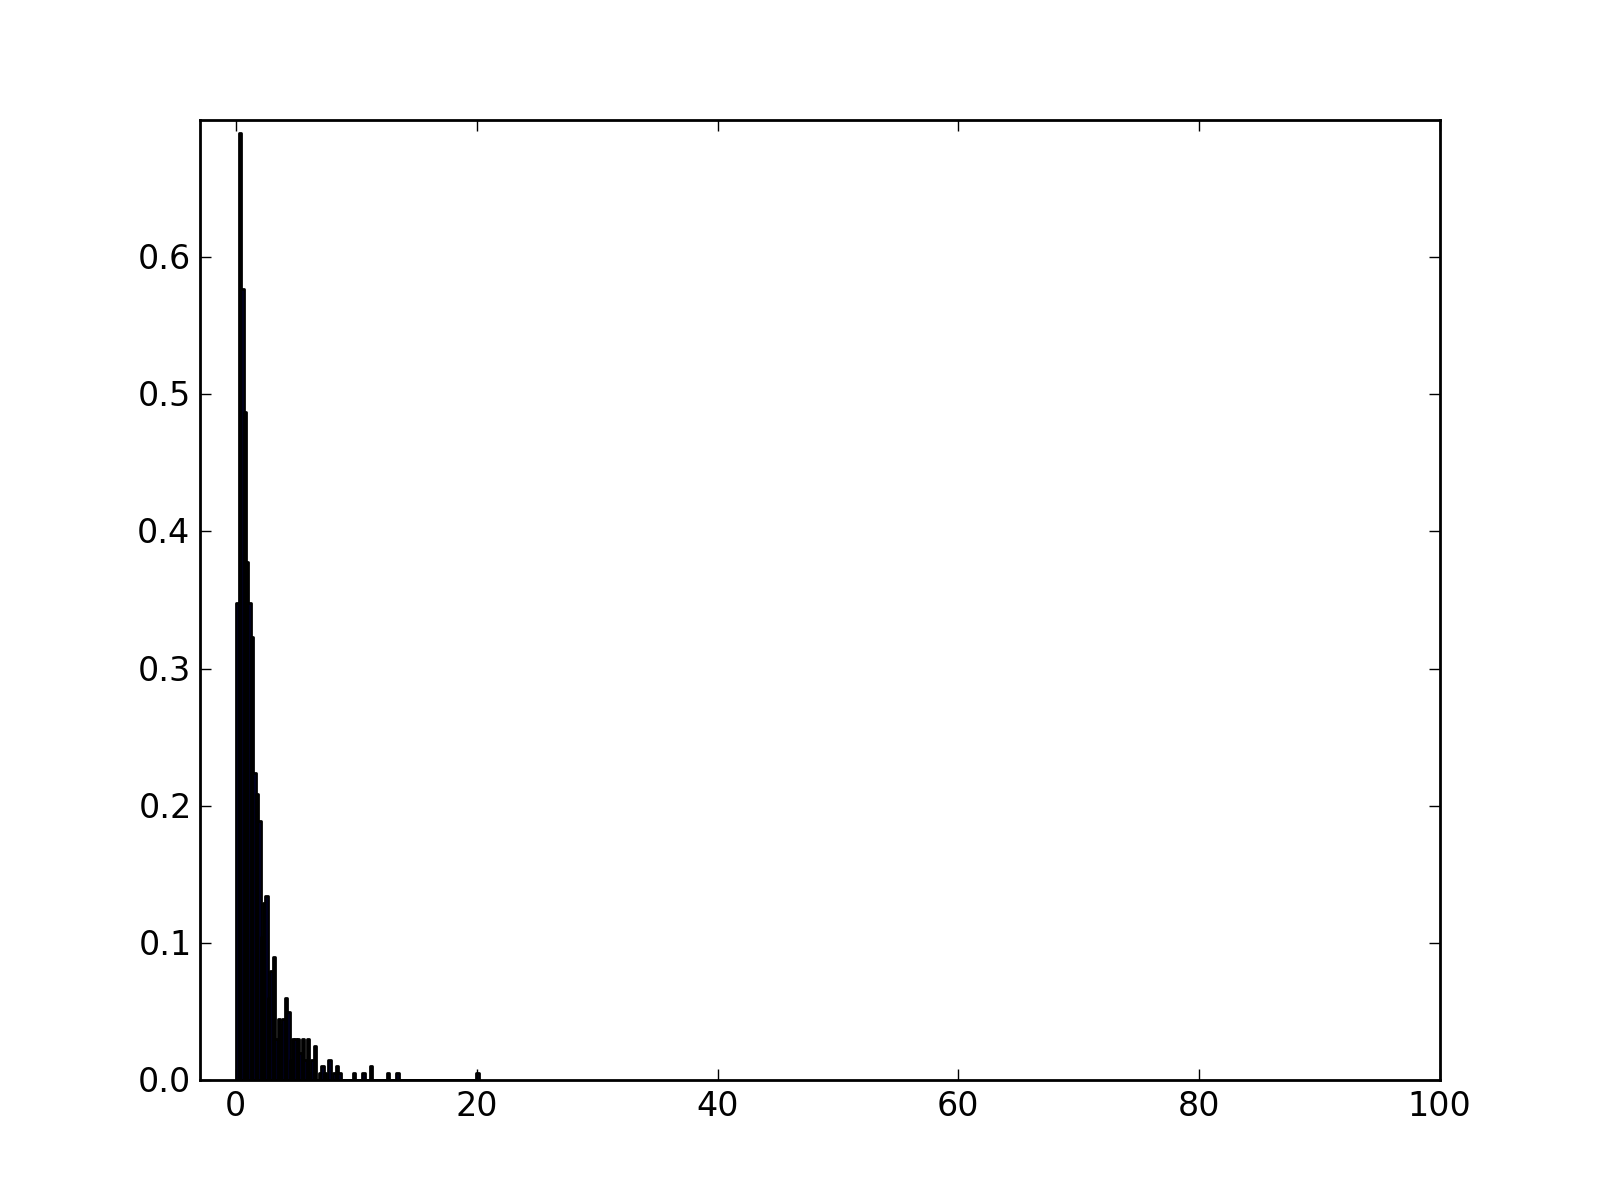
\includegraphics[width=0.6\textwidth]{fig/fig3.png}
\caption{Overlay of the FEM solution and $u(x)= \exp(3x)$ (top), and error $e(x) = u(x)-u_h(x)$ (bottom).}
\label{fig:fig3}
\end{figure}

\begin{table}
\centering
  \begin{tabular}{c | c | c | c | c}
k&   N &      h    &     L2    &     rate      \\ \hline
0&  101& 0.01000000& 0.0093932535&    --       \\ 
1&  201& 0.00500000& 0.0023604731&  1.9925489  \\
2&  401& 0.00250000& 0.00059221977&  1.9948715 \\ 
3&  801& 0.00125000& 0.00014831877&  1.9974315 \\ 
4& 1601& 0.00062500& 3.7113397e-05&  1.9986892
  \end{tabular}
\caption{Convergence analysis for FEM method with mixed BC.}
\label{tab:table3}
\end{table}


\section{Implementation notes}
The Python code associated with this report has 3 main classes: one computes the FEM solution, one creates the grid, and the last
one evaluates the solution and computes the norm. These classes can be found in ``femlib.py''. The main code is in ``hw03.py'',
and some utility functions and plotting command are found in $util.py$.
\end{document}
